\uuid{ovqT}
\exo7id{2633}
\auteur{debievre}
\organisation{exo7}
\datecreate{2009-05-19}
\isIndication{true}
\isCorrection{true}
\chapitre{Fonction de plusieurs variables}
\sousChapitre{Différentiabilité}

\contenu{
\texte{
Soit la fonction $f\colon\R^2\to\R$ d\'efinie par
$$
f(x,y)=\frac{xy^2}{x^2+y^2}, \quad (x,y)\not=(0,0)
$$
et $f(0,0)=0$.
}
\begin{enumerate}
    \item \question{Montrer que $f$ est continue et que,
quel que soit $v\in\R^2$, la d\'eriv\'ee directionnelle
 $D_vf(x,y)$ existe en chaque
$(x,y)\in\R^2$  mais que $f$ n'est pas diff\'erentiable en
$(0,0)$.}
\reponse{$\mathrm{lim}
_{\begin{smallmatrix} (x,y) \to (0,0)\\ (x,y) \ne (0,0) \end{smallmatrix}}
\frac{xy^2}{x^2+y^2}=\lim_{r\to 0}r \cos \varphi \sin^2 \varphi
$ 
existe et vaut z\'ero puisque $\cos \varphi \sin^2 \varphi$ est born\'e.
Par cons\'equent $f$ est continue \`a l'origine et donc partout.
Il est \'evident que la fonction $f$ est diff\'erentiable
en chaque point distinct de l'origine.
Soit $v=(a,b)\in\R^2$ non nul. Alors
\[
D_vf(0,0) = \left .\frac{d}{dt}\left(t\frac{ab^2}{a^2+b^2}\right)\right|_{t=0}=\frac{ab^2}{a^2+b^2}
\]
existe d'o\`u
$\frac{\partial f}{\partial x}(0,0)=0$ et
$\frac{\partial f}{\partial y}(0,0)=0$;
puisqu'il existe une d\'eriv\'ee directionnelle non nulle,
la fonction $f$ ne peut pas \^etre diff\'erentiable en $(0,0)$.}
    \item \question{La d\'eriv\'ee directionnelle $D_vf(0,0)$ 
est-elle lin\'eaire en $v$? Les droites
appartenant \`a la famille 
des droites passant par l'origine
et de vecteurs directeurs $(v, D_vf(0,0))\in\R^3$, forment-elles un plan? 
Expliquer comment on peut observer la r\'eponse sur la figure.}
\reponse{L'association $\R^2 \to \R,\ v \mapsto D_vf(0,0)$
n'est \'evidemment pas lin\'eaire
et les droites appartenant \`a la famille  des droites passant par l'origine
et de vecteurs directeurs $(v, D_vf(0,0))\in\R^3$ ne forment pas un plan.}
    \item \question{Le vecteur $v$ \'etant fix\'e, qu'est-ce qu'on peut dire de
la continuit\'e de $D_vf(x,y)$ en $(x,y)$?

{\center
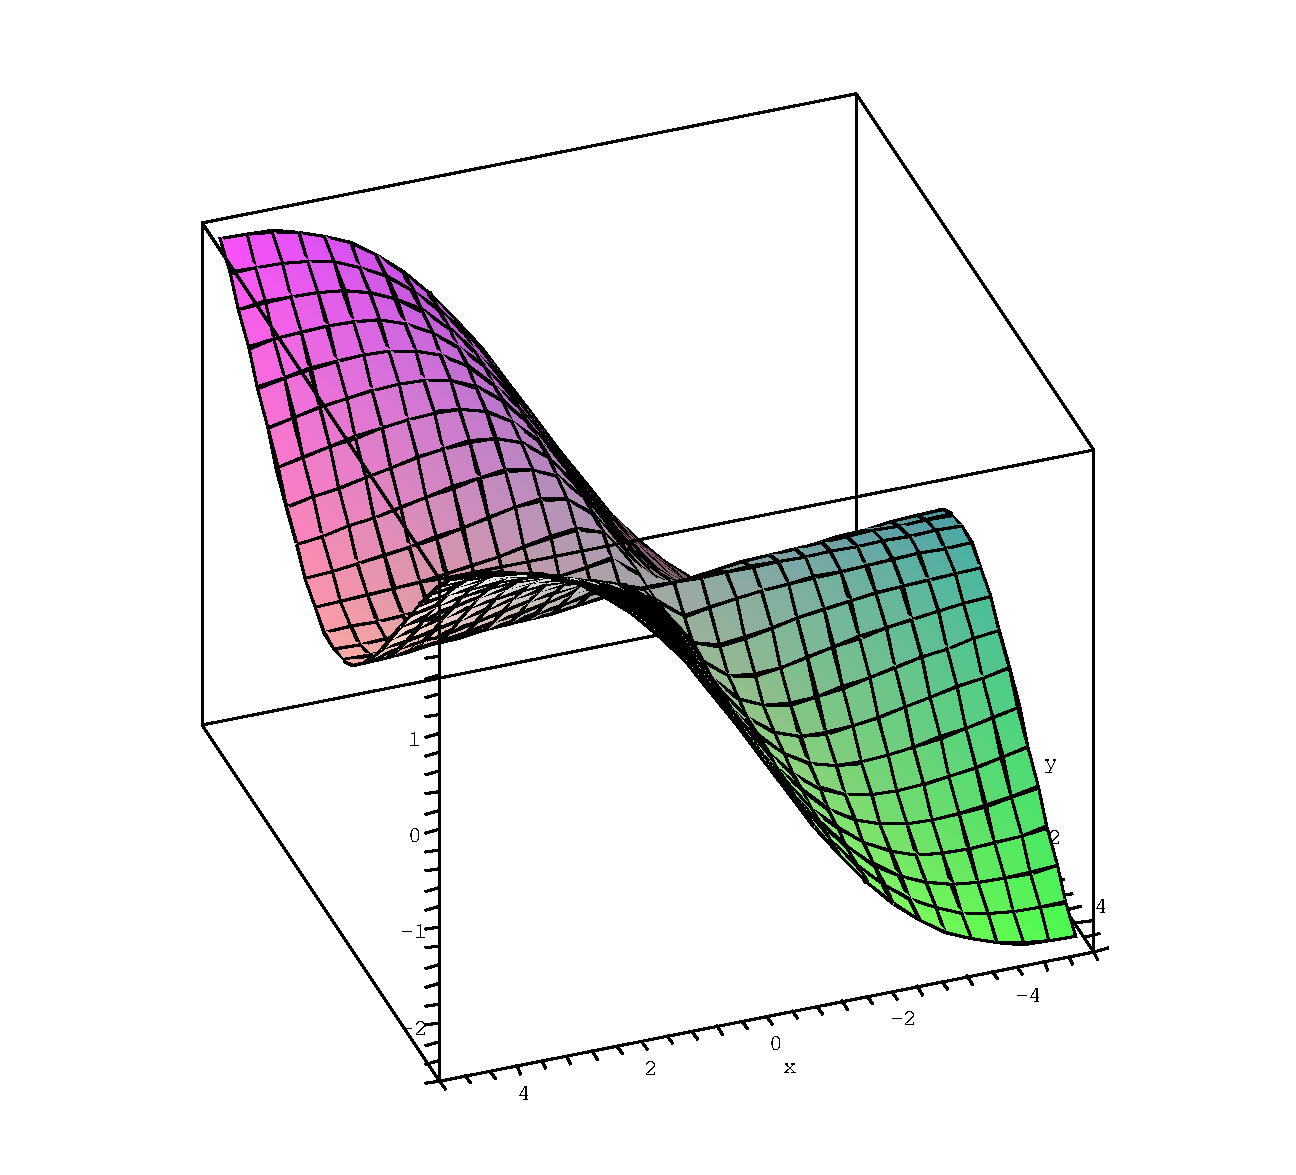
\includegraphics[height=6cm, keepaspectratio]{../images/img002633-1}
}}
\reponse{Dans $\R^2\setminus\{ (0,0)\}$, 
\begin{align*}
\frac{\partial f}{\partial x} &=\frac{y^2(x^2+y^2)-2x^2y^2}{(x^2+y^2)^2}
=\frac{y^4-x^2y^2}{(x^2+y^2)^2}=\sin^4 \varphi -\sin^2 \varphi \cos^2 \varphi
\\
\frac{\partial f}{\partial y} &=\frac{2xy(x^2+y^2) -2xy^3}{(x^2+y^2)^2}
=\frac{2x^3y}{(x^2+y^2)^2} = 2\sin \varphi \cos^3 \varphi
\end{align*}
d'o\`u, en coordonn\'ees polaires,
\[
D_vf(x,y)=D_vf(r \cos \varphi,r \sin \varphi)=
a(\sin^4 \varphi -\sin^2 \varphi \cos^2 \varphi)
+2b\sin \varphi \cos^3 \varphi 
\]
et, $\varphi$ \'etant fix\'e, 
\[ 
\mathrm{lim}_{r \to 0}D_vf(r \cos \varphi,r \sin \varphi)=
a(\sin^4 \varphi -\sin^2 \varphi \cos^2 \varphi)
+2b\sin \varphi \cos^3 \varphi .
\]
Par cons\'equent,
$D_vf(x,y)$ n'est pas continu en $(x,y)$ sauf peut-\^etre si $a=0$.
Par exemple, avec $\sin \varphi =1$, on trouve
\[ 
\mathrm{lim}_{r \to 0}D_vf(0,r)=a 
\]
et $a \ne \frac{ab^2}{a^2+b^2}$ sauf si $a=0$.
Si $a=0$, la d\'eriv\'ee directionnelle $D_v$ est la d\'eriv\'ee partielle
$\frac{\partial f}{\partial y}$ et, $\varphi$ \'etant fix\'e,
\[ 
\mathrm{lim}_{r \to 0}D_vf(r \cos \varphi,r \sin \varphi)=
2b\sin \varphi \cos^3 \varphi 
\]
ce qui n'est pas  nul si $\sin \varphi \cos \varphi$ ne l'est pas.
Puisque $\frac{\partial f}{\partial y}(0,0)=0$, la d\'eriv\'ee partielle
$\frac{\partial f}{\partial y}$ n'est continue en $(0,0)$ non plus.}
\indication{Pour les majorations, utiliser les coordonn\'ees
polaires $(r,\varphi)$ dans le plan.
Distinguer tout de suite les parties triviales des parties non triviales
de l'exercice.}
\end{enumerate}
}
